\documentclass{beamer}
\usetheme{default}
%\usetheme{pittsburgh}
\usecolortheme{albatross}

%###############################################################################
%#
%# Saját színek:
%#
\definecolor{todobgszin}{rgb}{0.64000,0.78000,0.22000}
\definecolor{todofrszin}{rgb}{0.00000,0.50000,0.00000}
\definecolor{background}{rgb}{0.00000,0.29412,0.49804}
%#
%###############################################################################

\setbeamercolor{normal text}{fg=white}
\setbeamertemplate{navigation symbols}{} % Navigációs ikonok off

\usepackage[T1]{fontenc}
\usepackage[utf8]{inputenc}
\usepackage[english,magyar]{babel}

\usepackage{hyperref}
\usepackage{color}
\usepackage{graphics}

\usebackgroundtemplate{

\includegraphics[width=\paperwidth, height=\paperheight]{figures/background.jpg}
}

% Néhány konstans deklarációja:
\newcommand{\vikszerzo}{Nádudvari György}
\newcommand{\vikszerzomail}{ulqp9p@gmail.com}
\newcommand{\vikkonzulens}{Gönczy László}
\newcommand{\vikkonzulensmail}{gonczy@mit.bme.hu}
\newcommand{\vikcim}{Virtualizált környezetek teljesítmény elemzése vizuális adatelemzés módszerekkel}

%###############################################################################
%#
%# Footer definíció a szokásos címek beírásához.
%#
%# Csúnya hacket tartalmaz!!!
%# A "{footline}{#1}" utáni \textcolorral egy háttérszínnel megegyező "y"
%# karaktert írunk ki, hogy ne ugráljanak a dobozok a diákon.
%# Ha ez elmarad, akkor az alapvonal alá nyúló karaktereket (pl. g, y stb.)
%# tartalmazó stringek esetén eltérő magasságban lesz a footer, mint azoknál
%# amelyek csak az alapvonalra illeszkedő karaktereket tartalmaznak.
%#
\newcommand{\setfootline}[1]{\setbeamertemplate{footline}{\setbeamercolor{footline}{fg=white}\begin{beamercolorbox}[sep=1cm,wd=\textwidth,ht=1cm,left]{footline}{#1}\textcolor{background}{y}\end{beamercolorbox}}}
%#
%###############################################################################

%###############################################################################
%#
%# Saját eszközök:
%#
\newcommand{\todo}[1]{\fcolorbox{todofrszin}{todobgszin}{\emph{TODO: #1}}}
\newcommand{\angolul}[1]{\foreignlanguage{english}{#1}}
%#
%###############################################################################

\hypersetup{
    bookmarks=true,            % show bookmarks bar?
    unicode=true ,             % non-Latin characters in Acrobat’s bookmarks
    pdftitle={\vikcim},        % title
    pdfauthor={\vikszerzo},    % author
    pdfnewwindow=true,         % links in new window
    colorlinks=true,           % false: boxed links; true: colored links
    linkcolor=black,           % color of internal links
    citecolor=black,           % color of links to bibliography
    filecolor=black,           % color of file links
    urlcolor=black             % color of external links
}

\title{\vikcim}
\author{\vikszerzo \\ {\footnotesize <~\vikszerzomail~>} \\ [0.5cm] {\small Konzulens: \vikkonzulens} \\ {\footnotesize <~\vikkonzulensmail~>}}
\date{2012. december 07.}

\begin{document}

\newcommand{\slidecim}{}

\section{Cím lap - \vikcim}
\begin{frame}[plain]
\titlepage
\todo{Zoli?}
\end{frame}

\renewcommand{\slidecim}{Miről is lesz szó?}
\section{\slidecim}
\setfootline{\todo{Keep floyding}}
\begin{frame}[t]
\frametitle{\slidecim}
\begin{itemize}
    \item Az adatelemzés általános áttekintése
    \item A vizualizáció előnyei, hátrányai
    \item VMware virtualizációs technológia
    \item Virtualizációs metrika adathalmazok vizualizációja
    \item Összefoglalás
\end{itemize}
\end{frame}

\renewcommand{\slidecim}{Mi az, hogy adatelemzés?}
\section{\slidecim}
\setfootline{\todo{Keep floyding}}
\begin{frame}[t]
\frametitle{\slidecim}
\todo{•}
\end{frame}

\renewcommand{\slidecim}{Az adatvizualizáció előnyei, hátrányai}
\section{\slidecim}
\setfootline{\todo{Keep floyding}}
\begin{frame}[t]
\frametitle{\slidecim}
\todo{•}
\end{frame}

\renewcommand{\slidecim}{Egy példa - Zipf eloszlás megjelenése a kutatócsoport honlapjának látogatottságában}
\section{\slidecim}
\setfootline{\todo{Keep floyding}}
\begin{frame}[t]
\frametitle{\slidecim}
\begin{figure}[!ht]
\centering
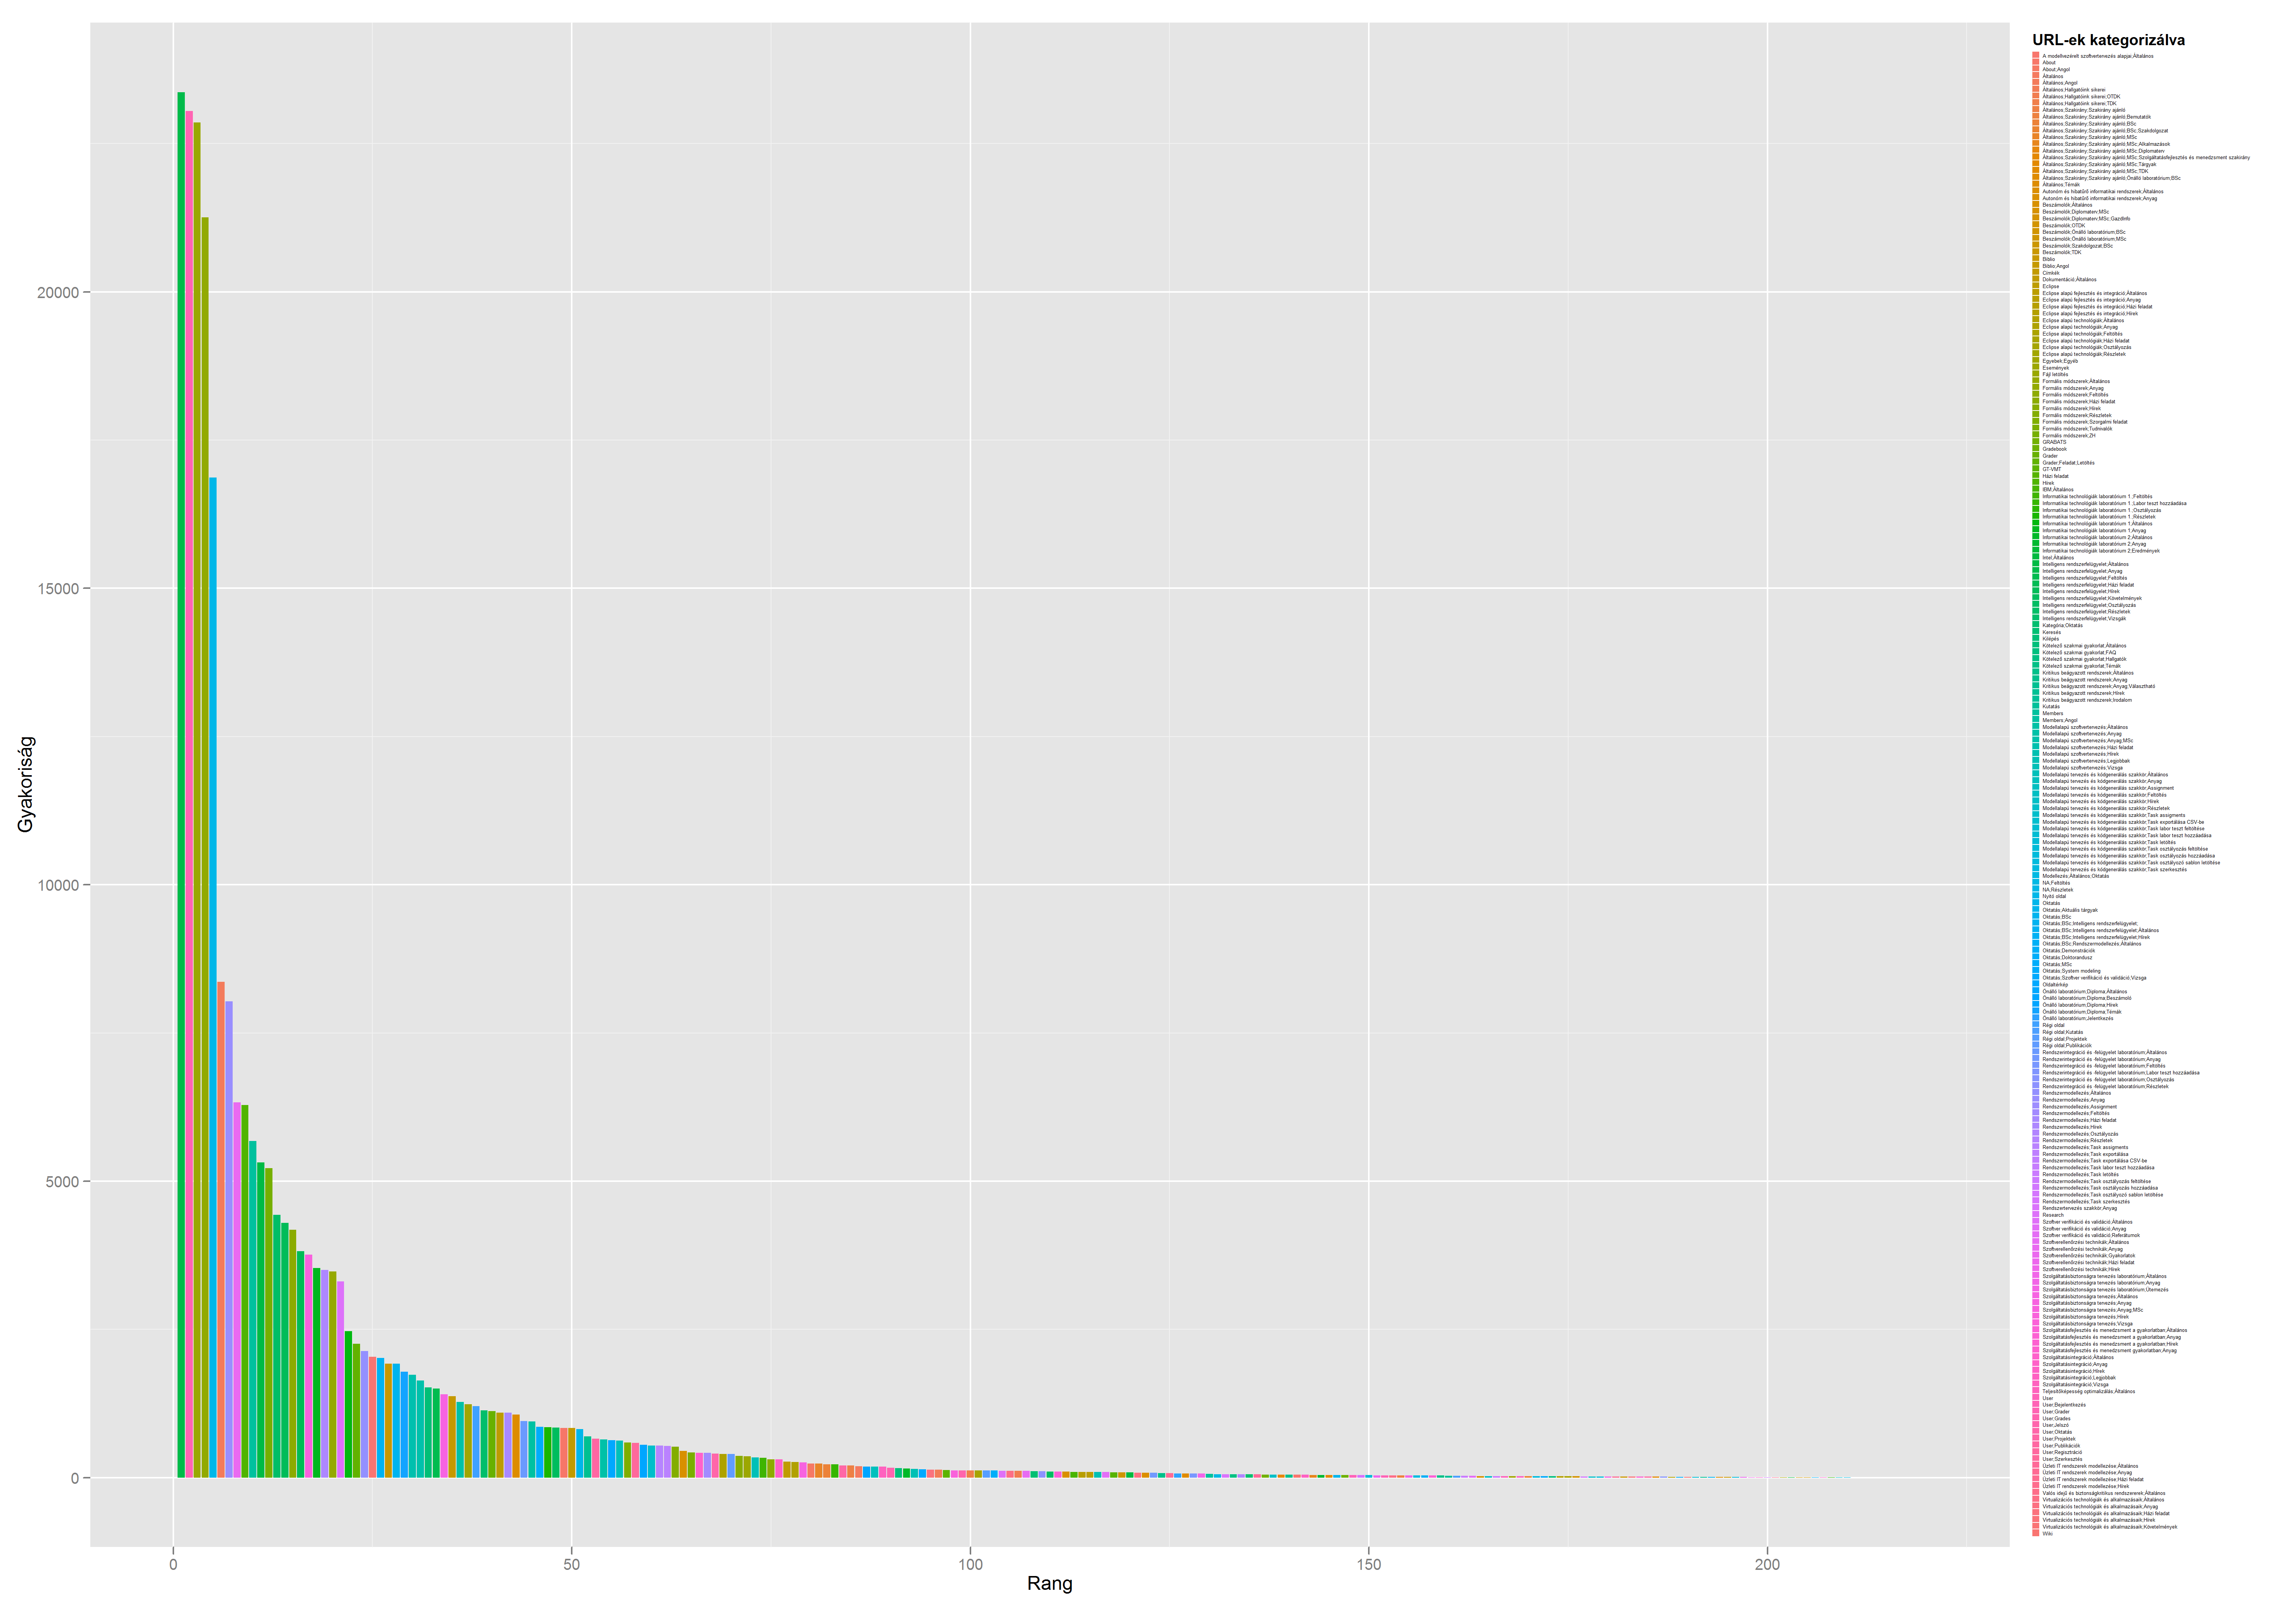
\includegraphics[height=68mm, keepaspectratio]{figures/zipf_url_views_cat_plot.png}
\end{figure}
\end{frame}

\renewcommand{\slidecim}{Még egy példa - Zipf eloszlás megjelenése a Rendszermodellezés tárgy aloldalainak látogatottságában}
\section{\slidecim}
\setfootline{\todo{Keep floyding}}
\begin{frame}[t]
\frametitle{\slidecim}
\begin{figure}[!ht]
\centering
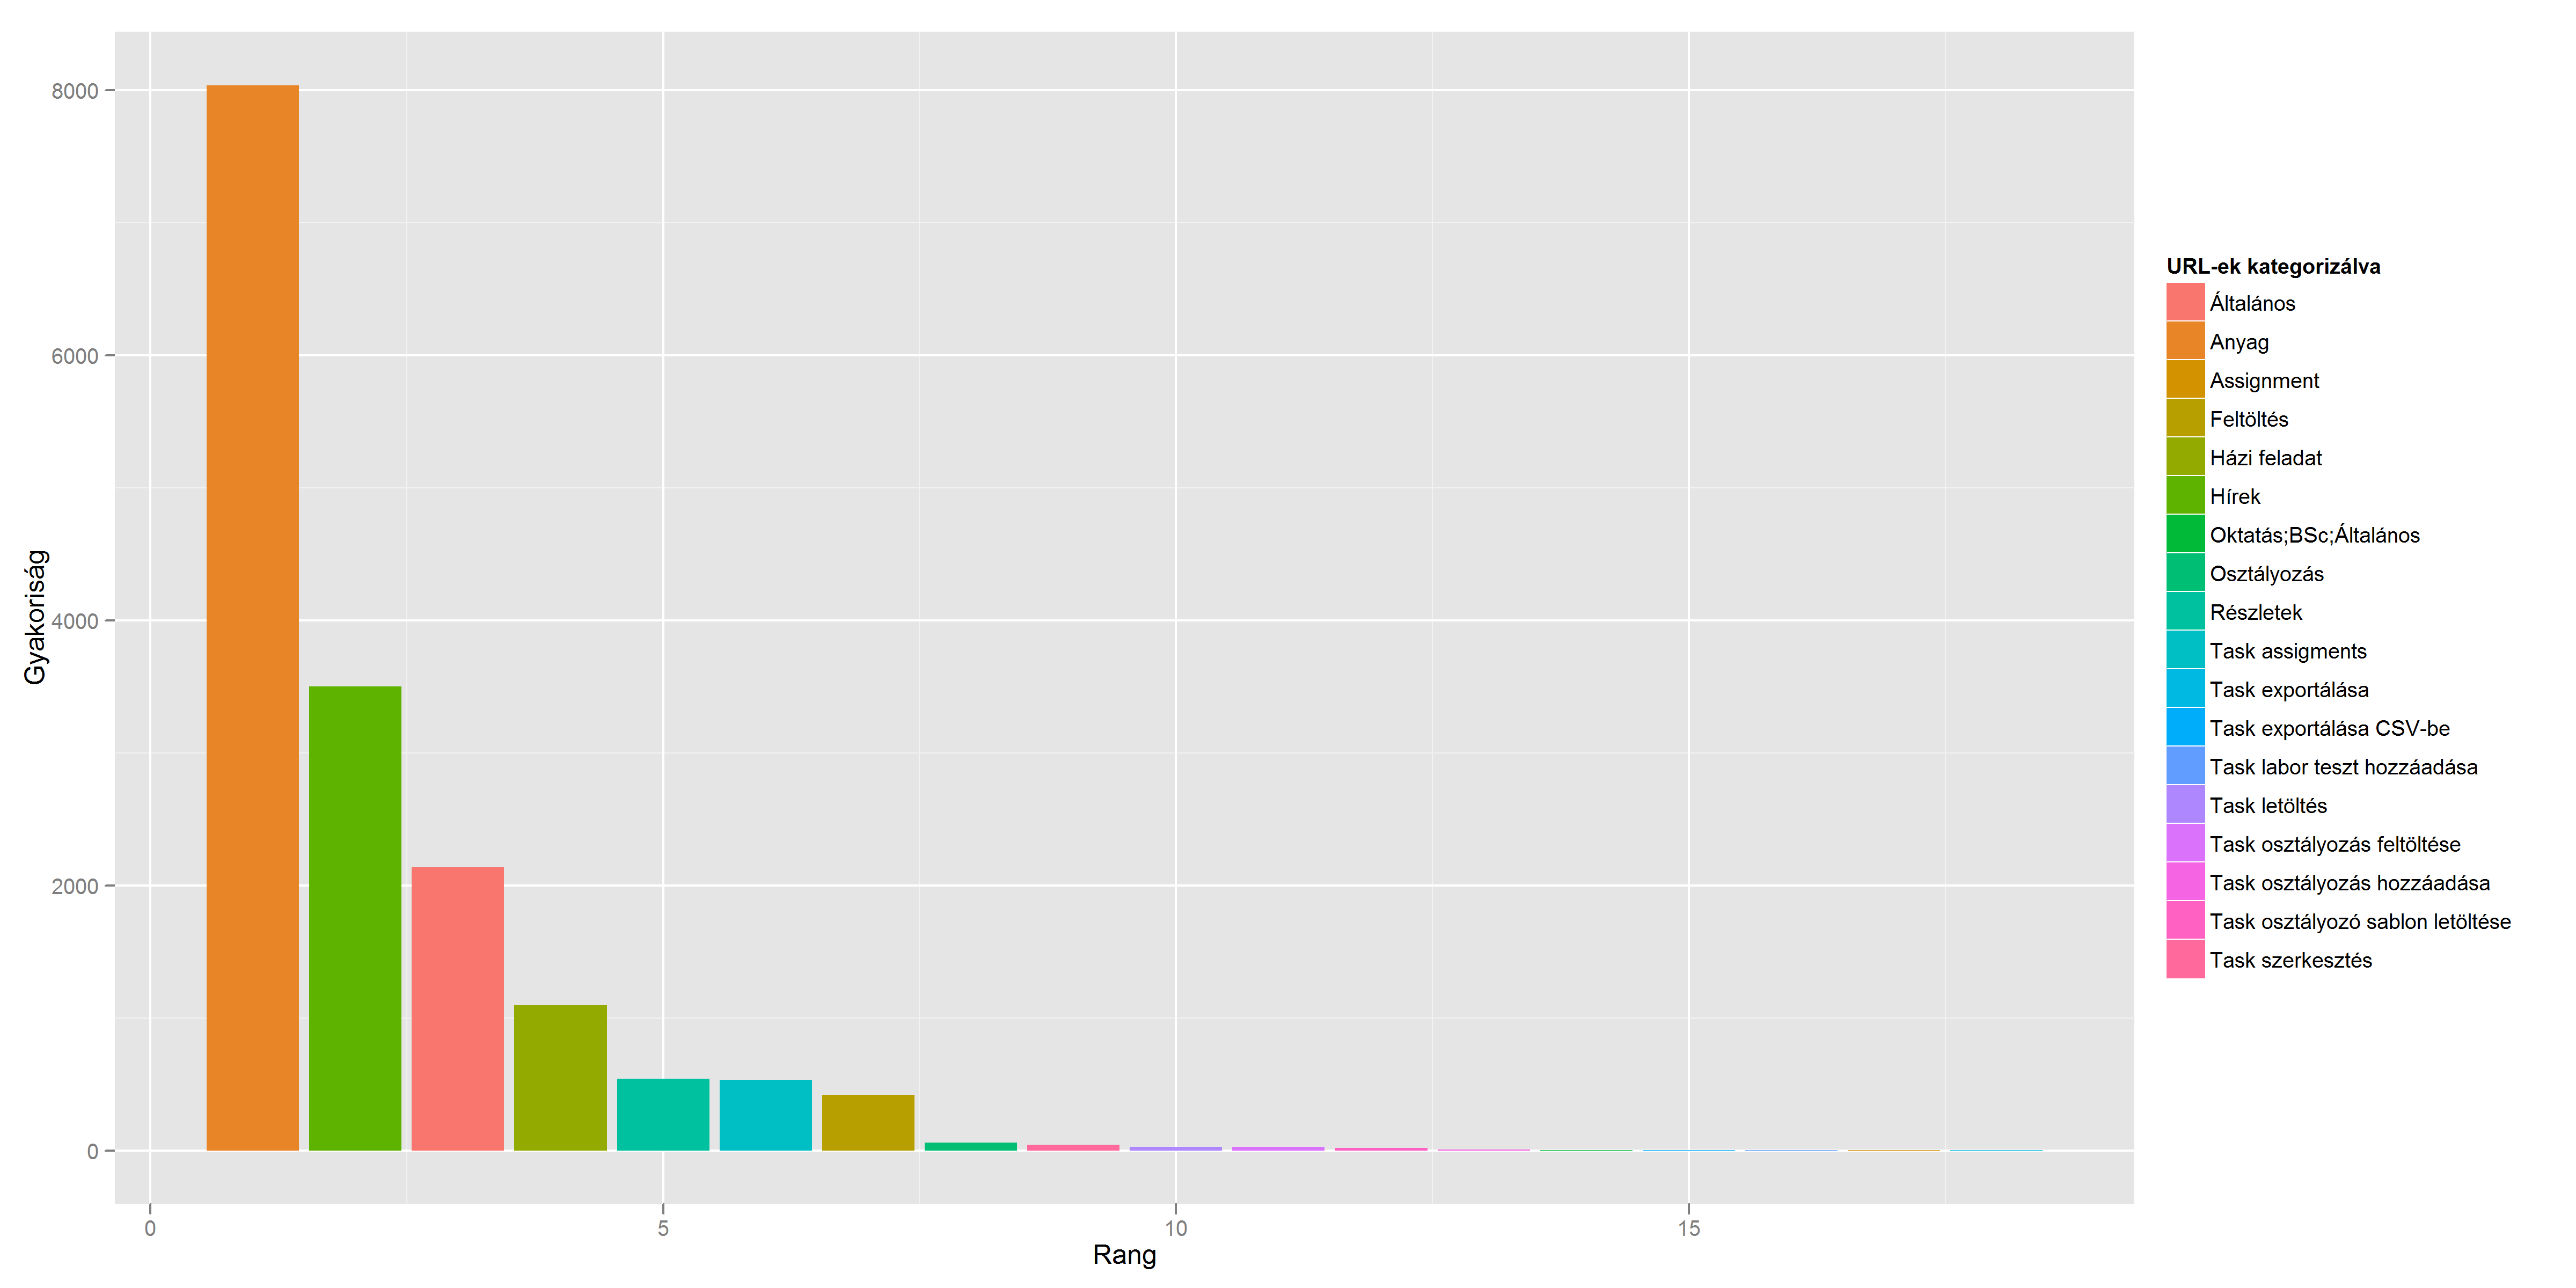
\includegraphics[width=110mm, keepaspectratio]{figures/zipf_remo_url_views_cat_plot.png}
\end{figure}
\end{frame}

\renewcommand{\slidecim}{A VMware virtualizációs technológia}
\section{\slidecim}
\setfootline{\todo{Keep floyding}}
\begin{frame}[t]
\frametitle{\slidecim}
\todo{•}
\end{frame}

\renewcommand{\slidecim}{Virtualizációs infrastruktúra metrikák vizualizációja}
\section{\slidecim}
\setfootline{\todo{Keep floyding}}
\begin{frame}[t]
\frametitle{\slidecim}
\todo{•}
\end{frame}

\renewcommand{\slidecim}{Összefoglalás - Elért eredmények}
\section{\slidecim}
\setfootline{\todo{Keep floyding}}
\begin{frame}[t]
\frametitle{\slidecim}
\begin{itemize}
\item Megismert technológiák, eljárások:
    \begin{itemize}
        \item R statisztikai szkript nyelv alapjai
        \item Adattisztítás, adatelemzés alapjai
        \item VMware virtualizációs infrastruktúra metrikák
    \end{itemize}
\item Továbblépési lehetőségek:
    \begin{itemize}
        \item Naplóállomány feldolgozásának, tisztításának automatizálása
        \item Virtualizációs infrastruktúrák teljesítmény problémáinak előrejelzése, automatikus felderítése
    \end{itemize}
\end{itemize}
\end{frame}

\section{Kérdések}
\setfootline{\angolul{Is There Anybody Out There?}}
\begin{frame}[c]
\frametitle{}
\begin{center}
\huge{\textbf{Kérdések?}}\\
\begin{figure}[!ht]
\centering

\includegraphics[width=20mm, keepaspectratio]{figures/questions.png}
\end{figure}
\end{center}
\end{frame}

\section{Vége}
\setfootline{\angolul{Comfortably Numb}}
\begin{frame}[c]
\frametitle{}
\begin{center}
\huge{\textbf{Köszönöm a figyelmet!}}
\end{center}
\end{frame}

\end{document}
